%webimpl.tex
This section describs the work of implementing the web interface in Servlets.

\subsubsection{Mockups}
To get startet at series of mockups was created, to get an idea of the geneal look and feel of the website. An example of this is shown in \autoref{fig:mockSelectProfile}, the rest can be found in \autoref{app:Mock}.

\begin{figure}[htbp]
	\centering
		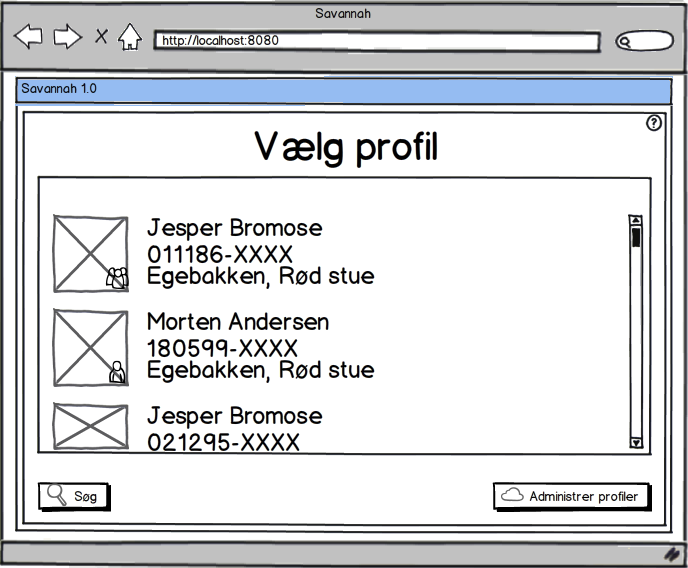
\includegraphics[width=1.00\textwidth]{images/mockSelectProfile.png}
	\caption{A mockup of profile selection}
	\label{fig:mockSelectProfile}
\end{figure}

\subsubsection{Programming languages}
The web interface uses four different languages: Servlets, HTML, JavaScript, and Cascading Style Sheets (CSS). The Servlets are used responisble for database access, and generation of both the HTML code and JavaScript, and the CSS is used for for the graphic on each page. The HTML is used for making the elements on the webpages, and the JavaScript is sued to add some dynamic to a generated HTML side.

\subsubsection{Structure}
The structure of each Servlets page is seen in \autoref{fig:webStruct}
\begin{figure}
	\centering
		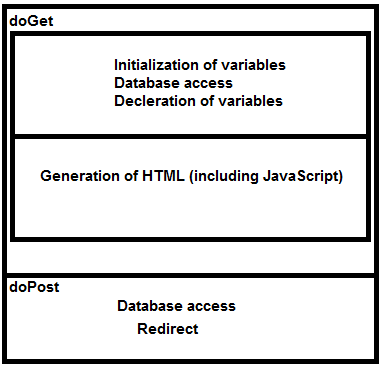
\includegraphics{images/webStruct.png}
	\caption{General structure of Servlets}
	\label{fig:webStruct}
\end{figure}

When a webpage is first loaded, it access the \code{doGet} code, and executes the code within. After this there are three scenarios:
\begin{description}
	\item[Scenario 1] The user click a link, and is sent to a new page.
	\item[Scenario 2] The user submits a \code{form} with \code{doGet} method. 
	\item[Scenario 3] The user submits a \code{form} with \code{doPost} method.
\end{description}

In scenario 1, the current pages do not do anything else but send the user to the new page, which executes the code in its \code{doGet} code. In scenario 2 the \code{form} structure dictates what happens: It can either redirect to itself, and execute the \code{doGet} method again \autoref{code:getRedirectSelf}, or redirect to a new page and execute the \code{doGet} method on that, see \autoref{code:getRedirectNew}.

\begin{lstlisting}[language=Java,label=code:getRedirectSelf,caption=A form which redirect to its own get method]
	@WebServlet("/DeleteTags")
	
	/**
	 * @see HttpServlet#doGet(HttpServletRequest request, HttpServletResponse response)
	 */
	protected void doGet(HttpServletRequest request, HttpServletResponse response) throws ServletException, IOException {
	
	out.println("<center><form method='GET' name='formName' action='DeleteTags'>");
	}
\end{lstlisting}

\begin{lstlisting}[language=Java,label=code:getRedirectNew,caption=A form which redirect to its own get method]
	@WebServlet("/DeleteTags")
	
	/**
	 * @see HttpServlet#doGet(HttpServletRequest request, HttpServletResponse response)
	 */
	protected void doGet(HttpServletRequest request, HttpServletResponse response) throws ServletException, IOException {
	
	out.println("<center><form method='GET' name='formName' action='NewPage'>");
	}
\end{lstlisting}

Secnario 3, has almost the same code as \autoref{code:getRedirectSelf} and \autoref{code:getRedirectNew}, with the excpetion that the \code{method='POST'}.

In generalt the \code{form} is build as \code{<form method='POST/GET' name='NameOfForm' action='WhichPageToExecuteCodeFrom>}.

\subsubsection{Database access}
The read data from the database is handled by Java code in each of the Servlets, the code is shown in \autoref{code:readDatabase}. To update attributes in the database, the \code{stmt.executeQuery} is used, with the appropriate SQL script.  To delete data, instead of \code{stmt.executeQuery} a \code{PreparedStatement} is created, this is executed with by calling \code{int i = ps.executeUpdate();} which will give either a OK code (0) or and error code. 

\begin{lstlisting}[language=Java,label=code:readDatabase,caption=Code to read data from the database]
public void readData()
{
String dataVar;
Connection con = null;
Statement stmt = null;
ResultSet rs = null;
try {
   Class.forName("com.mysql.jdbc.Driver"); //Use this driver to access the database
   con = DriverManager.getConnection("jdbc:mysql://DatabaseAddress", "Username", "Password"); //Instansiate the connection
   stmt = con.createStatement(); //Instansiate stmt
   rs = stmt.executeQuery("SQL query"); //Executes the SQL query and get the result store in RS
   //As long rs contains data, read it!
   while (rs.next()) { 
      String name = rs.GetString("Name"); //Get a string attribute
      int number = rs.GetString("Number"); //Get a int attribute
}
//Error handeling
catch (SQLException e) 
{		
   throw new ServletException("Servlet Could not display records.", e);
} 
catch (ClassNotFoundException e) 
{			
   throw new ServletException("JDBC Driver not found.", e);
}
//Make sure the connection is closed, no matter what 
finally {
   try {
      if (rs != null) {
         rs.close();
         rs = null;
      }
      if (stmt != null) {
         stmt.close();
         stmt = null;
      }
      if (con != null) {
         con.close();
         con = null;
      }
   } 
catch (SQLException e) 
{			
}
}

\end{lstlisting}

\subsubsection{Generation of the web page}
The generation of the web page, is done within the servlet, using a \code{PrintWriter}. This is instansiated by cy calling \code{PrintWriter out = response.getWriter();}, and used to write the HTML code by calling \code{out.println("HtmlCode");} which will generate a web page, with only THAT code visible. \code{out} can furthermore be used to write both JavaScript and CSS.

The CSS however is not written within any of the Servlets, instead is i located in a seperate file \verb+/WebContent/CSS/SavannahStyle.css+ and is included in the HTML by \code{ "<link rel='stylesheet' type='text/css' href='CSS/SavannahStyle.css' />"}


\subsubsection{Exchange of data}
When a Servlet submits a form, the data is sent differently depending on the \code{form} method. A \code{GET} method will send the data as a part of the URL thus make it visible for the user, as seen in\autoref{code:URLLINK}, where as the \code{POST} method does not make it visible.

\subsubsection{\code{Form} data}
To access the data from the \code{form}, this needs a name. The name it set by the \code{name} attribute in the \code{input} element. The type of data sent from the \code{form} depends on the type of element.
\begin{description}
	\item[\code{Text},\code{Password} and \code{TextField}] The value of these fields are of the type string, and contains the value entered
	\item[\code{RadioButton}] All \code{RadioButton}s with the same name, sends the value of the selected \code{RadioButton}
	\item[\code{CheckBox}] All \code{CheckBox}es with the same name sends the value of each checked box.
	\item[\code{DropdownBox}] Sends the value of the selected item
	\item[\code{ListBox}] Send the value of all the selected items as a string array
\end{description}

\begin{lstlisting}[language=Java,label=code:URLLINK,caption=URL with visible parameters]
http://www.xoxoxoxox.com/servlet/ServletName?var1=value&var2=value&var3=value
\end{lstlisting}

To be able to retrieve the data sent by the form the \code{request.getParameter()} method is used. An example of this is shown in \autoref{code:getDataInPost}.

\begin{lstlisting}[language=Java,label=code:getDataInPost,caption=How to read parameters]
	@WebServlet("/PseudoClass")
	/**
	 * @see HttpServlet#doPost(HttpServletRequest request, HttpServletResponse response)
	 */
	protected void doPost(HttpServletRequest request, HttpServletResponse response) throws ServletException, IOException {
		String myVar = request.getParameter("FieldName"); //Get single Value
		String[] myVarArray = request.getParameterValues("FieldName") //Get string array
	}
\end{lstlisting}

\subsubsection{Current limitatio}
When uploading a picture, a \code{file} type is used to select the local file on the hard disk. The \code{file} has a security restricting, which makes it impossible to set a default value for the field. This is due to the fact, that if it was possible, it could be used to send a file from the visitor of a web page's hard disk, without the visitor has any knowledge of it\cite{noFile}. Futhermore it was not straight forward to get the path of a selected file, again due to security restrictions, but this turned out to be possible by the use of JavaScript, the code is seen in \autoref{code:myHack}, and adding parameter \code{onChange="readURL(this);"} to the \code{file} field.

\begin{lstlisting}[language=HTML,label=code:myHack,caption=Hack to load file from \code{file} box]
var reader = new FileReader();+
reader.onload = function(e) 
   {
      document.billedet.src  = e.target.result;
   };

function readURL(input)
   {
      if(input.files && input.files[0])
      {
         reader.readAsDataURL(input.files[0]);
      }
      else 
      {
         document.billedet.src = "";
      }
   }
\end{lstlisting}

A navigation diagram of the web site is shown in \autoref{fig:WebNav}, and shows that all pages and information can be accessed within three clicks.

\begin{figure}
	\centering
		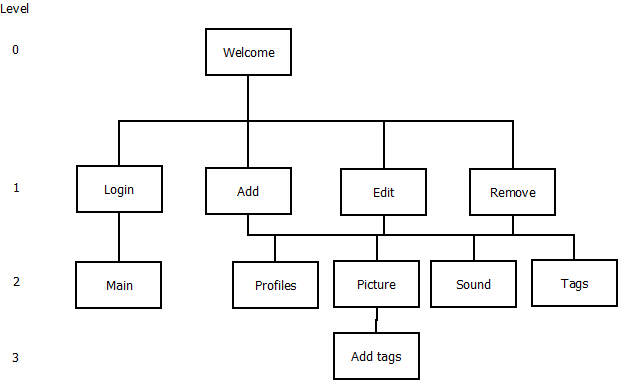
\includegraphics[width=1.00\textwidth]{images/WebNav.png}
	\caption{Navigation diagram for the web site}
	\label{fig:WebNav}
\end{figure}
